\documentclass[10pt]{beamer}
\usetheme{Goettingen}

\usepackage[utf8]{inputenc}
\usepackage[T1]{fontenc}
\usepackage[french]{babel}

%\usepackage{algpseudocode}

%\usepackage{algorithm}
%\usepackage{algorithmic}
\newcommand{\kw}[1]{\textrm{#1}}

\usepackage{forest}

%\usepackage{scrextend}
%\changefontsizes{7.5pt}

\usefonttheme[onlymath]{serif}

\usepackage{xcolor}
\usepackage{graphicx} 
\usepackage{amsmath}
\usepackage{amssymb} % pour les ensembles NN
\usepackage{mathrsfs} % pour les hypothèses de récurrences \PP
\setlength{\unitlength}{1mm}
%\usepackage{enumitem}
\usepackage{cancel}

\usepackage{neuralnetwork}

%\usepackage{fancyhdr}
\usepackage{multicol}

\usepackage{booktabs}
\usepackage{tabularx}
\usepackage{array,collcell}
\newcommand\AddLabel[1]{%
  \refstepcounter{equation}% increment equation counter
  (\theequation)% print equation number
  \label{#1}% give the equation a \label
}
\newcolumntype{M}{>{\hfil}X<{\hfil}} % mathematics column
%\newcolumntype{M}{>{\hfil$\displaystyle}X<{$\hfil}} % mathematics column
%\newcolumntype{L}{>{\collectcell\AddLabel}r<{\endcollectcell}}
\renewcommand\tabularxcolumn[1]{m{#1}}% for vertical centering text in X column

\usepackage{tikz}
\usetikzlibrary{calc, shapes, shadows}

\usepackage{tkz-graph}
\tikzset{EdgeStyle/.append style = {->}}
\tikzset{LabelStyle/.style= {draw,
fill = white,
text = black}}

\newcommand*\keystroke[1]{%
  \tikz[baseline=(key.base)]
    \node[%
      draw,
      fill=white,
      drop shadow={shadow xshift=0.25ex,shadow yshift=-0.25ex,fill=black,opacity=0.75},
      rectangle,
      rounded corners=2pt,
      inner sep=1pt,
      line width=0.5pt,
      font=\scriptsize\sffamily
    ](key) {#1\strut}
  ;
}

\newcommand*\circled[1]{\tikz[baseline=(char.base)]{
            \node[shape=circle,draw,inner sep=1pt] (char) {#1};}}
            
\usepackage{etoolbox} % for \ifnumcomp
\usepackage{listofitems} % for \readlist to create arrays

\tikzset{>=latex} % for LaTeX arrow head
\colorlet{myred}{red!80!black}
\colorlet{myblue}{blue!80!black}
\colorlet{mygreen}{green!60!black}
\colorlet{mydarkred}{myred!40!black}
\colorlet{mydarkblue}{myblue!40!black}
\colorlet{mydarkgreen}{mygreen!40!black}
\tikzstyle{node}=[very thick,circle,draw=myblue,minimum size=22,inner sep=0.5,outer sep=0.6]
\tikzstyle{connect}=[->,thick,mydarkblue,shorten >=1]
\tikzset{ % node styles, numbered for easy mapping with \nstyle
  node 1/.style={node,mydarkgreen,draw=mygreen,fill=mygreen!25},
  node 2/.style={node,mydarkblue,draw=myblue,fill=myblue!20},
  node 3/.style={node,mydarkred,draw=myred,fill=myred!20},
}
\def\nstyle{int(\lay<\Nnodlen?min(2,\lay):3)} % map layer number onto 1, 2, or 3



% ensembles N,Z,Q,D,R,C
\DeclareMathOperator{\NN}{\mathbb{N}}
\DeclareMathOperator{\ZZ}{\mathbb{Z}}
\DeclareMathOperator{\QQ}{\mathbb{Q}}
\DeclareMathOperator{\DD}{\mathbb{D}}
\DeclareMathOperator{\RR}{\mathbb{R}}
\DeclareMathOperator{\CC}{\mathbb{C}}
\DeclareMathOperator*{\argmax}{\arg\!\max}

\title{TIPE 2024}
\subtitle{Apprendre à une intelligence artificielle à jouer à Snake en utilisant un algorithme génétique}
\author{Marilou Bernard de Courville}
\institute{Lycée Charlemagne}
\date{\today}

\setbeamertemplate{footline}[frame number]


\begin{document}
 
\begin{frame}
    \titlepage
\end{frame}

%\begin{frame}
%    \frametitle{Table des matières}
%    \tableofcontents
%\end{frame}

\section{Introduction}

\begin{frame}
\frametitle{Introduction}
\framesubtitle{Problématique et pertinence au regard du thème de l'année}

\begin{itemize}

\item \textbf{Le jeu de Snake:} piloter un serpent sur une grille dans le but de
manger des pommes, sans rentrer dans les murs ni se replier sur 
soi-même.

\item \textbf{Objectif:} mettre en place une intelligence
artificielle pouvant jouer au jeu de Snake, apprenant de manière autonome.

\item \textbf{Le moyen d'y parvenir:} utiliser un algorithme génétique,
qui s'inspire de l'évolution naturelle.

\end{itemize}

\end{frame}

\section{Le principe}

\subsection{Le jeu de Snake}


\begin{frame}
\frametitle{Le jeu de Snake}
\framesubtitle{Brève histoire et règles du jeu}

\begin{columns}[T]
\begin{column}{0.70\textwidth}
\footnotesize
\textbf{Origines:} borne d'arcade \textit{Blockade}, créée par Gremlin en 1976, popularisé par Nokia en 1997 sur mobile 

\vspace{0.5cm}

\textbf{Règles du jeu:}  

\begin{itemize}
\footnotesize
\item Le serpent débute avec une longueur initiale sur un échiquier entouré d'un mur et contenant une pomme.
\item L'objectif est de le faire grandir en mangeant des pommes.
\item Chaque pomme consommée augmente sa longueur d'une unité et en fait apparaître une nouvelle à un emplacement aléatoire.
\item Le joueur dirige le serpent à l'aide des touches directionnelles du clavier \keystroke{$\leftarrow$}\keystroke{$\uparrow$}\keystroke{$\downarrow$}\keystroke{$\rightarrow$}.
\item Le jeu se termine si le serpent heurte un mur ou son propre corps.
\item Le score du joueur est égal au nombre de pommes mangées.
\end{itemize}


\end{column}
\begin{column}{0.24\textwidth}
\begin{figure}
\centering
\vspace{-1cm}\hspace{-0.6cm}
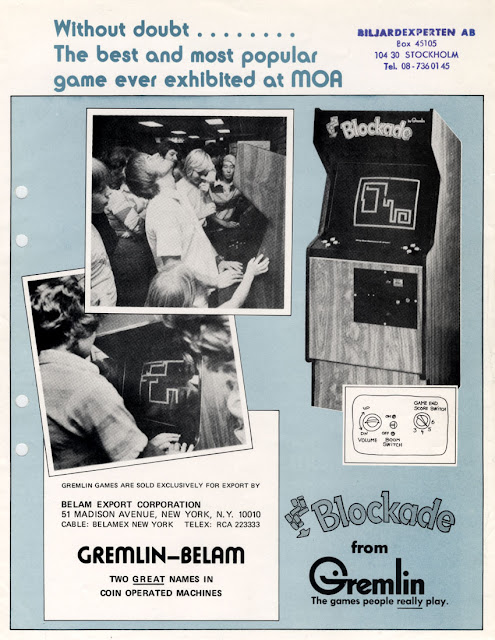
\includegraphics[width=1\textwidth]{blockade.jpg}
\end{figure}

\begin{figure}
\vspace{-0.8cm}\hspace{-0.6cm}
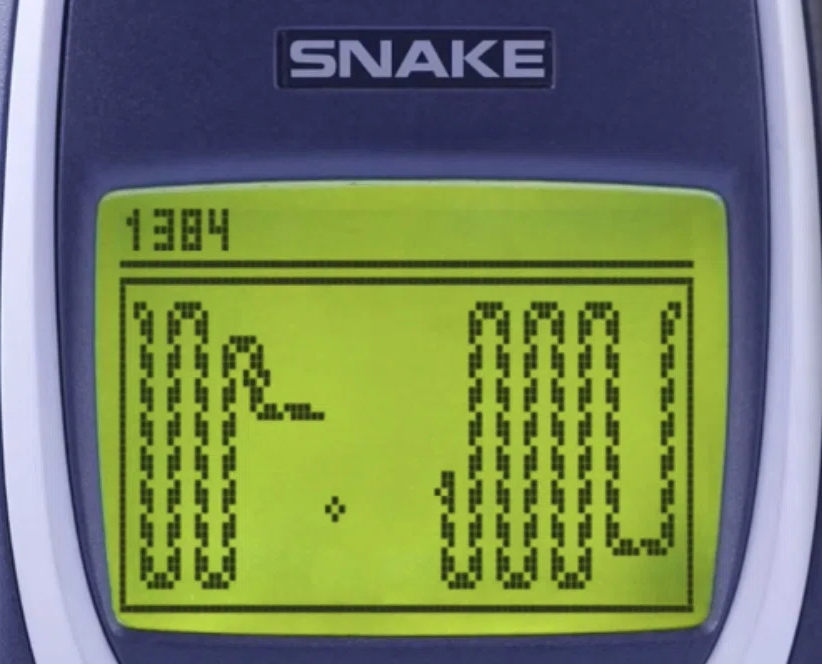
\includegraphics[width=0.97\textwidth]{snake_nokia.png}
\end{figure}  

\begin{figure}
\vspace{-1.1cm}\hspace{-0.6cm}
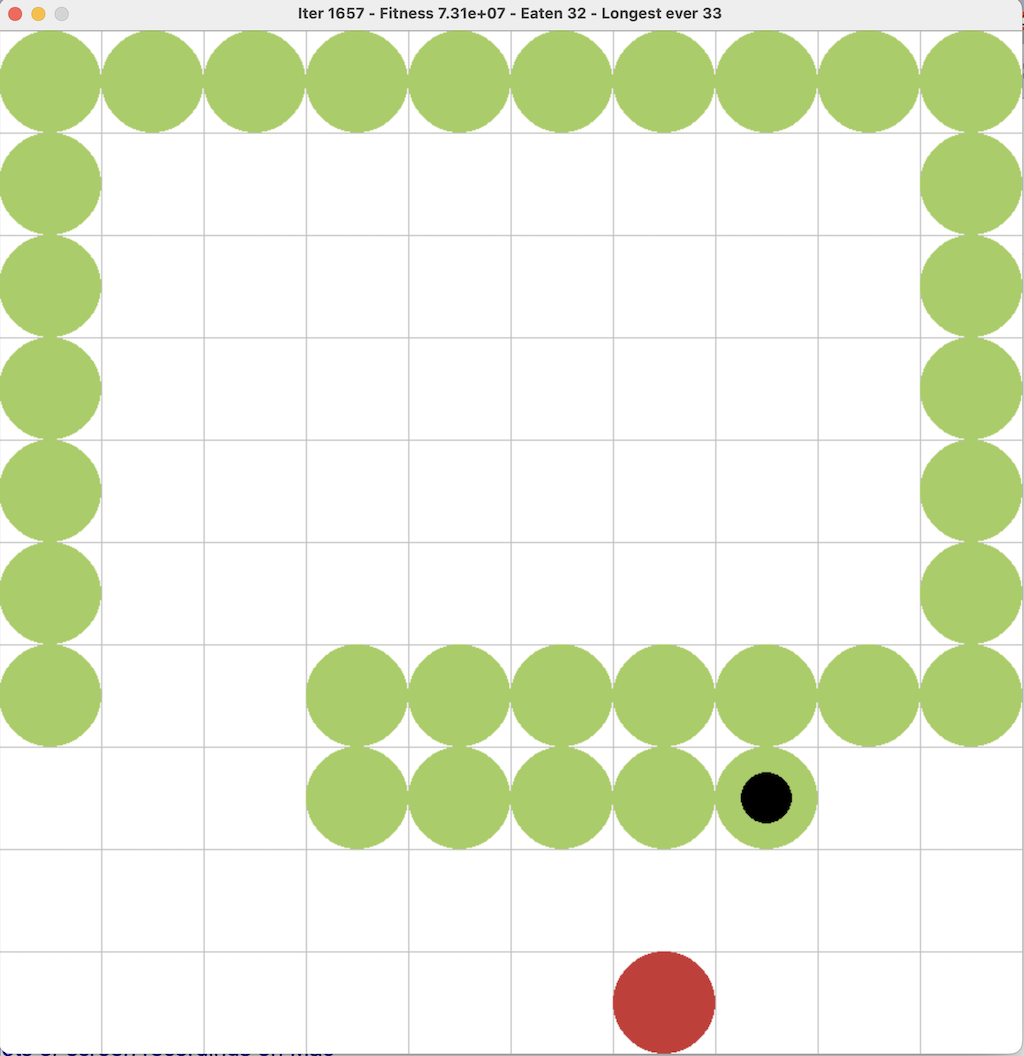
\includegraphics[width=1\textwidth]{snake_game.png}
\end{figure}



\end{column}
\end{columns}
\end{frame}

\subsection{L'algorithme génétique}

\begin{frame}
  \frametitle{Le principe de l'algorithme génétique}
  \framesubtitle{Histoire, fonctionnement et applications de l'algorithme}    
  
  \begin{itemize}

    \item \textbf{Origines:} développé par John Holland dans les années 1970

    \item \textbf{Principe:} s'inspirer de l'évolution naturelle pour
    résoudre des problèmes d'optimisation

    \item \textbf{Fonctionnement:} on part d'une population aléatoire, on les fait évoluer en appliquant des opérateurs
    génétiques (sélection, crossover, mutation)

    \item \textbf{Applications:} problème du voyageur de commerce, problèmes de décision (optimisation dans les banques), NASA et Sony pour des déplacements de robots, automatisation des tests d'application par Motorola
    
    \item \textbf{Ici:} application ludique, on applique cet algorithme à un réseau neuronal pour qu'il joue à Snake
   

  \end{itemize}  
  \end{frame}
  

\subsection{Les réseaux neuronaux}

\begin{frame}

  \frametitle{Le principe des réseaux neuronnaux}
  \framesubtitle{Histoire et principe}
  
  \begin{itemize}
    
    \item \textbf{Origines:} Warren S. McCulloch et Walter Pitts, \textit{A logical calculus of the ideas immanent in nervous activity}, 1943, compare les neurones à seuil binaire à la logique booléenne puis Frank Rosenblatt, \textit{The perceptron: a probabilistic model for information storage and organization in the brain}, 1958, introduit la notion de poids
    
    \item \textbf{Principe:} 3 couches de n\oe uds qui transmettent des informations à la couche suivante suivant s'ils sont activés et leurs poids, s'appuient sur l'entraînement pour être plus précis
    
    \item \textbf{Fonctionnement:} on code des "yeux" au serpent, ie. on prend en compte ce qu'il voit devant lui, et le réseau neuronal va analyser ces données pour que le serpent tourne ou pas.
    
    \item \textbf{Lien avec l'algorithme génétique:} les différents poids associés aux neurones vont être transmis ou non aux enfants

  \end{itemize}

  \end{frame}

  \section{La théorie}


  \subsection{L'algorithme génétique}
  
  \begin{frame}
    \frametitle{Le fonctionnement de l'algorithme génétique}
  \end{frame}
  
  \begin{frame}
    \frametitle{Le Théorème de Holland}
  \end{frame}
  
  \subsection{Les réseaux neuronaux}
  
  \begin{frame}
    \frametitle{Le fonctionnement des réseaux de neurones}
  
    % check https://tex.stackexchange.com/questions/153957/drawing-neural-network-with-tikz
    % check https://tex.stackexchange.com/questions/153957/drawing-neural-network-with-tikz
  
    % incompatibility to be treated by https://tex.stackexchange.com/questions/420448/error-illegal-parameter-number-in-definition-of-iterate i.e. replace # by ####
    
  
  \end{frame}

\section{L'algorithme appliqué au jeu de Snake}

\subsection{Relation algorithme génétique et réseaux de neurones}

\begin{frame}
  \frametitle{Comment algorithme génétique et réseaux de neurones sont reliés}
\end{frame}

\subsection{L'importance d'une fonction de fitness: trouver la bonne stratégie}

\begin{frame}
  \frametitle{Trouver la stratégie gagnante avec la fonction fitness}
\end{frame}

\subsection{Les résultats}

\begin{frame}
  \frametitle{Les résultats}
\end{frame}

\section{Conclusion}

\begin{frame}
  \frametitle{Conclusion}
\end{frame}

\end{document}
